%
% Documento: Resultados Esperados
%

\chapter{Resultados Preliminares}

A partir de uma análise sobre qualidade de \textit{software}, métricas de qualidade e fundamentos teóricos do funcionamento do CSS, construiu-se uma pesquisa exploratória, em forma de um questionário, para identificação dos aspectos mais relevantes no processo de manutenção de uma folha de estilo e das características do código fonte que estão relacionadas a sua qualidade.

\section{Construindo o questionário}
Elaborou-se o questionário com os seguintes objetivos:

\begin{itemize}
	\item Identificar os aspectos da linguagem que mais impactam na legibilidade do código;
	\item Identificar os parâmetros que definem qualidade de código no ponto de vista dos entrevistados;
	\item Identificar aspectos mais custosos para manutenção;	
\end{itemize}

A partir da coleta das respostas, pode-se analisar os pesos de cada aspecto de qualidade do código CSS em função da manutenibilidade do estilo. Identificando as maiores ocorrências de efeitos colaterais, definindo quais são as técnicas para manter legibilidade mais utilizadas e quais aspectos de organização do código são mais relevantes.

\begin{figure}[!htb]
	\centering
	\caption{Exemplo de questão aplicada no questionário.}
	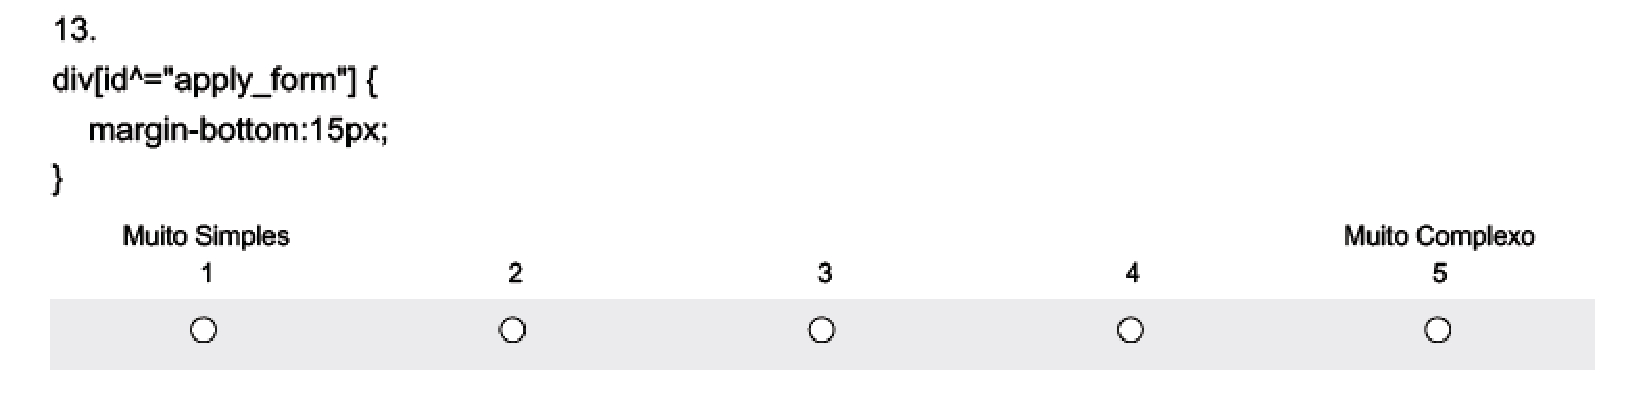
\includegraphics[width=1\textwidth]{./04-figuras/questionario_q13}
	\fonte{próprio autor}
	\label{fig:questionario_q13}
\end{figure}

Viu-se necessária a avaliação da complexidade de alguns aspectos da linguagem, a partir do ponto de vista do profissional, então o questionário (\autoref{chap:apendiceA}) foi construído com uma seção onde é avaliado, com base em um trecho de código (\autoref{fig:questionario_q13}), a dificuldade de se dar manutenção, cada trecho foi elaborado de acordo com um aspecto da linguagem que possam causa algum tipo de complicação. Esses aspectos foram escolhidos de acordo com as ponderações e experiência do autor, com base nos estudos realizados.

A dificuldade atribuída por cada pessoa a um determinado conjunto de regras e propriedades, é subjetiva e depende fortemente da experiência do individuo. Portanto construiu-se o questionário com perguntas visando a classificação do respondente de acordo com o seu nível de conhecimento, a partir dessa classificação será possível ponderar as respostas de acordo com o nível dos respondentes.

\section{Resultados do Questionário}

O questionário (\autoref{chap:apendiceA}) somou um total de vinte e sete (27) respostas, este número de respostas pode ser atribuído à permeabilidade dos meios de divulgação. Mesmo com um pequeno número de respostas, pôde-se executar uma análise a partir dos resultados da pesquisa. 

Durante os estudos para construção do questionário foram levantas as seguintes hipóteses:

\begin{itemize}
	\item \textbf{(h0)} A manutenção de folhas de estilo não é um trabalho trivial, podendo ocorrer efeitos colaterais durante esta etapa;
	\item \textbf{(h1)} O tamanho da folha de estilo é inversamente proporcional à manutenibilidade;
	\item \textbf{(h2)} Seletores com alta especificidade prejudicam a manutenção da folha de estilo;
	\item \textbf{(h3)} O uso correto de classes, com nomes coerentes, pode ser benéfico para a manutenção;
	\item \textbf{(h4)} A herança de propriedade é um fator causador de efeitos colaterais na etapa de manutenção;
	\item \textbf{(h5)} Seletores de alta complexidade prejudicam na manutenção;
	\item \textbf{(h6)} Regras inutilizadas;
\end{itemize}

O questionário teve então o intuito de validar essas hipóteses, de modo a confirmá-las ou refutá-las. Com uma série de perguntas exploratórias e as específicas, para determinar um valor de escala para os atributos específicos da linguagem.

\subsection{Nível de proficiência}

A primeira questão do questionário (\autoref{chap:apendiceA}) foi desenvolvida com o intuito de classificar os conhecimentos de cada respondente, para assim determinar-se o seu nível de proficiência. Essa classificação permitiu que os pesos definidos por cada respondente fosse ponderado de acordo com seu nível de proficiência.

Para esta classificação utilizamos os seguintes critérios para as funcionalidades do CSS.

\begin{quadro}
	\centering
	\caption{Classificação das características do CSS e nível de proficiência}
	\label{my-label}
	\begin{tabular}{|l|l|l|}
		\hline
		\textbf{Iniciante}                                                                         & \textbf{Imtermediário}                                                                                                             & \textbf{Avançado}                                                                        \\ \hline
		\begin{tabular}[c]{@{}l@{}}Localidade\\ Agrupamento\\ Aninhamento\\ Box Model\end{tabular} & \begin{tabular}[c]{@{}l@{}}Herança\\ Transformation\\ Transition\\ Pseudo classes\\ Pseudo elementos\\ Especificidade\end{tabular} & \begin{tabular}[c]{@{}l@{}}At-rules\\ Media queries\\ Animation e keyframes\end{tabular} \\ \hline
	\end{tabular}
	\fonte{Próprio autor}
\end{quadro}


\subsection{Visão Geral}

As respostas para o questionário formaram um conjunto de dados capaz de validar as hipóteses levantadas, não de forma definitiva, mas com dados suficientes para construção da métrica aqui proposta.

As questões propostas para identificar a qualidade do código CSS de maneira geral identificaram resultados diversos. Como na \autoref{fig:questionario_q2}, podemos verificar que mais de 90\% dos respondentes identificaram os elementos estruturais e a nomenclatura coerente para classes e identificadores (id's) como sendo imprescindíveis para qualidade da folha de estilo.

\begin{figure}[!htb]
	\centering
	\caption{Resultado da questão 2 do questionário \autoref{chap:apendiceA}.}
	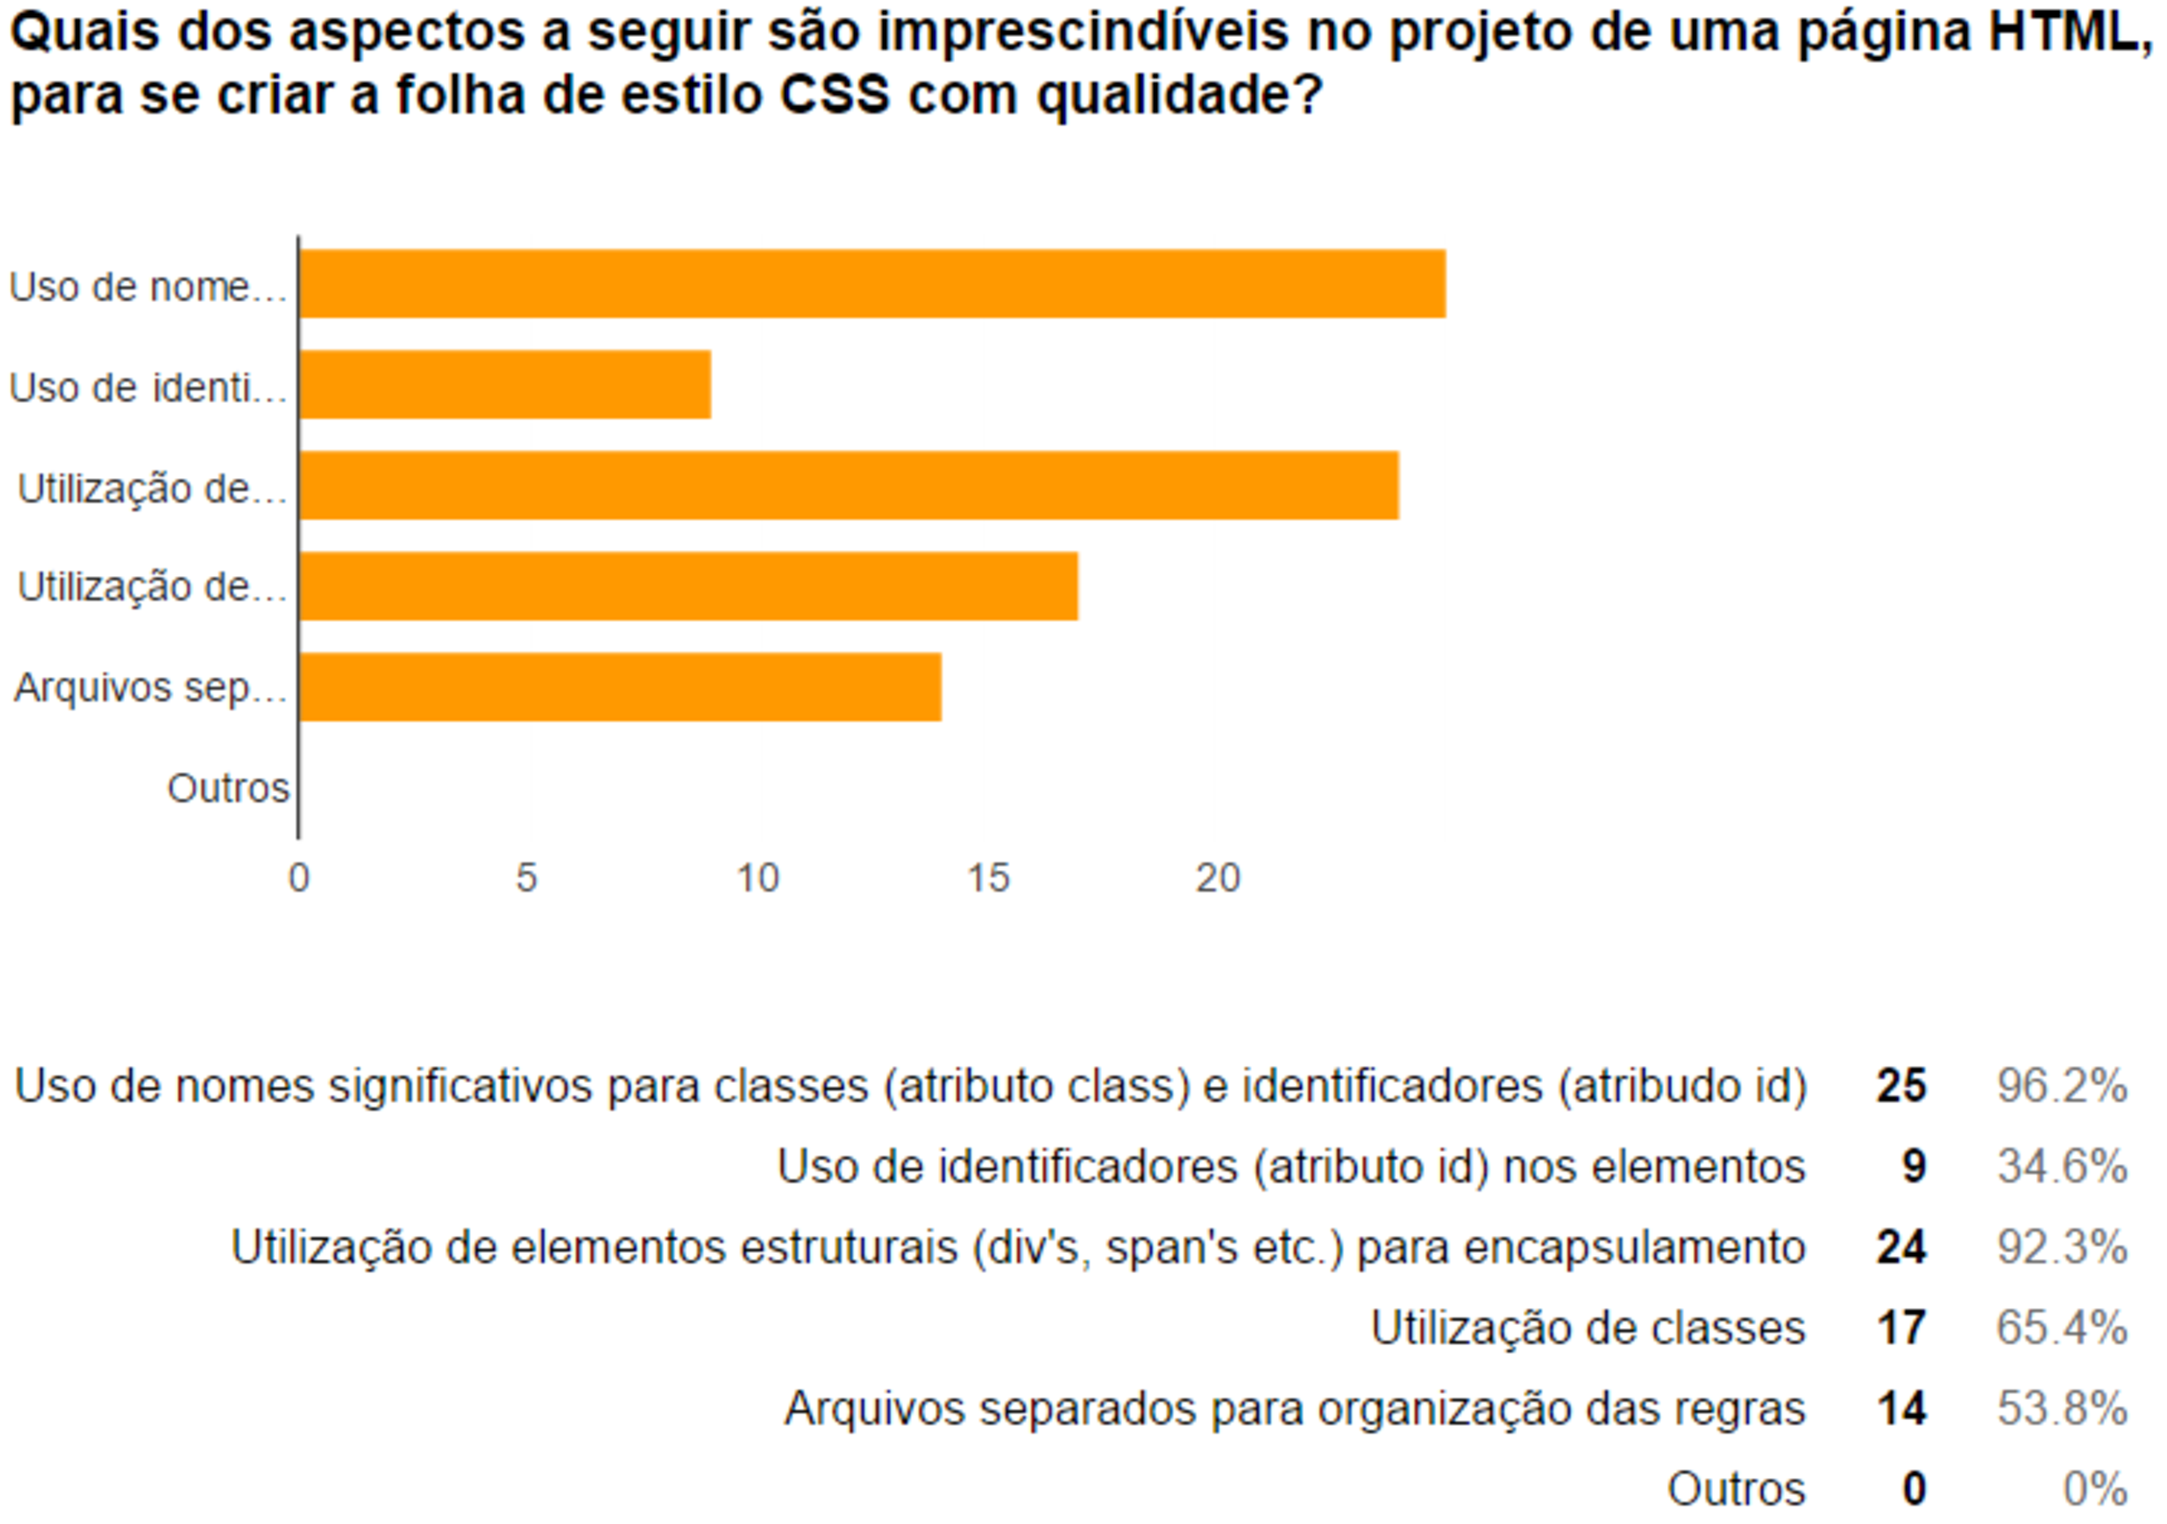
\includegraphics[width=0.9\textwidth]{./04-figuras/questionario_q2}
	\fonte{próprio autor}
	\label{fig:questionario_q2}
\end{figure}

Esta resposta corrobora com a hipótese h3, mostrando que a boa estruturação dos elementos do documento de conteúdo, impactam diretamente na construção da folha de estilo.

Na questão exposta em Figura \autoref{fig:questionario_q3} podemos notar os aspectos do CSS que interferem na qualidade do código CSS. Nota-se aqui que não houve unanimidade para esta questão, porém nota-se uma maior pontuação das questões de legibilidade do código, \textit{e.g.} organização em seções e modularidade do código.

\begin{figure}[!htb]
	\centering
	\caption{Resultado da questão 3 do questionário \autoref{chap:apendiceA}.}
	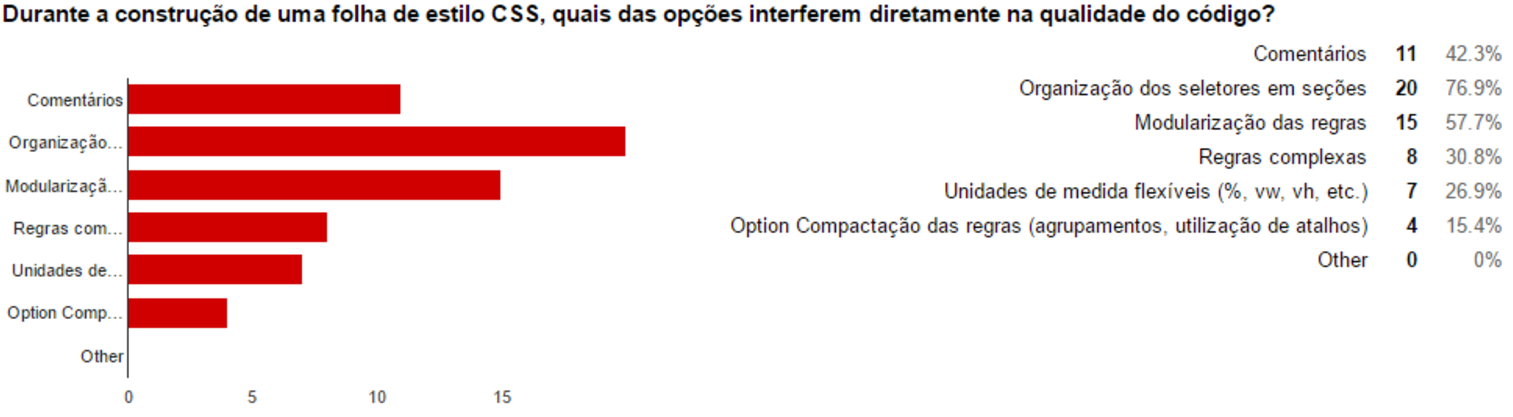
\includegraphics[width=0.9\textwidth]{./04-figuras/questionario_q3}
	\fonte{próprio autor}
	\label{fig:questionario_q3}
\end{figure}

Na Figura \autoref{fig:questionario_q9}, podemos verificar que o maior número de ocorrências de efeitos colaterais, para os respondentes, está na fase de manutenção do código. Esse resultado corrobora com a hipótese (h0).

\begin{figure}[!htb]
	\centering
	\caption{Resultado da questão 9 do questionário \autoref{chap:apendiceA}.}
	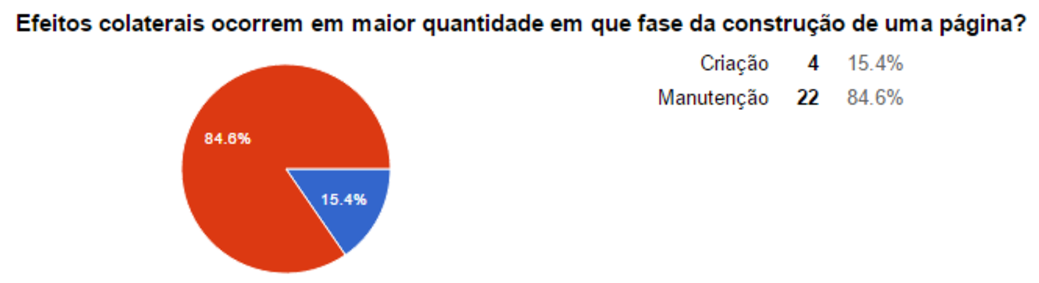
\includegraphics[width=0.9\textwidth]{./04-figuras/questionario_q9}
	\fonte{próprio autor}
	\label{fig:questionario_q9}
\end{figure}

Ainda sobre os efeitos colaterais, foi elaborada uma questão com objetivo de identificar quais são as propriedades do CSS que mais os causam. As respostas foram variadas e por isso não foi possível identificar um padrão a partir desta pesquisa. No entanto, as respostas com elementos semelhantes sempre tinham relação com definição de posicionamento e tamanho dos elementos (e.g.: position, margin, padding, display, width, z-index, float, etc). A partir das respostas obtidas podemos identificar os valores de manutenibilidade para os elementos que possuírem características de herança, prioridade e atuação semelhantes.

\subsection{Questões Exploratórias}

Algumas questões desse questionário tinham o objetivo de captar informações da experiência dos respondentes, a fim de identificar parâmetros que não foram cobertos pelo questionário. Algumas respostas agregaram valor à pesquisa, identificando esses pontos e mostrando algumas informações valiosas à cerca da qualidade da folha de estilo. 

Foi questionado quais são os pontos críticos que podem dificultar a manutenção, ou evolução, do código CSS. Das respostas obtidas podemos ver no \autoref{qd:openAnswers} aquelas que corroboram ou refutam as hipóteses levantadas.

\begin{quadro}[!htb]
	\centering
	\caption{Contribuição das respostas da questão 6 do questionário. (\autoref{chap:apendiceA})}
	\label{qd:openAnswers}
	\begin{tabular}{|l|c|c|}
		\hline
		\textbf{Resposta}                                                                                                                                                                                                                                                                                                                                                                                                                                                                                                            & \multicolumn{1}{l|}{\textbf{Corrobora}} & \multicolumn{1}{l|}{\textbf{Refuta}} \\ \hline
		Estilizar elementos sem classe, criar folhas de estilos muito extensas.                                                                                                                                                                                                                                                                                                                                                                                                                                                      & h1                                      &                                      \\ \hline
		CSS's que são atribuídos de forma mais genérica aos elementos.                                                                                                                                                                                                                                                                                                                                                                                                                                                                &                                         & h2                                   \\ \hline
		\begin{tabular}[c]{@{}l@{}}Regras complexas \\ Herança de valor de propriedade (valores,inherit, initial)\\ Aninhamento (seleção de elementos aninhados)\end{tabular}                                                                                                                                                                                                                                                                                                                                                  & h5                                      &                                      \\ \hline
		\begin{tabular}[c]{@{}l@{}}Utilização de nomes muitos genéricos para classes ou atributos.\\ A estilização que não é mais usada e fica no código.\end{tabular}                                                                                                                                                                                                                                                                                                                                                               & h3;h6                                   &                                      \\ \hline
		\begin{tabular}[c]{@{}l@{}}Regras para itens muito genéricos. \\ Utilização de !imporant. \\ Código repetido.\end{tabular}                                                                                                                                                                                                                                                                                                                                                                                                   & h6                                      & h2                                   \\ \hline
		Saber se um seletor está ou não sendo usado em algum parte do código.                                                                                                                                                                                                                                                                                                                                                                                                                                                        & h6                                      &                                      \\ \hline
		Seletores muito específicos.                                                                                                                                                                                                                                                                                                                                                                                                                                                                                                  & h2                                      &                                      \\ \hline
		\begin{tabular}[c]{@{}l@{}}Regras com seletores muito gerais, como classes e tags, \\ costumam provocar efeitos colaterais com mais frequência.\\ Acho que para poder escrever regras desse tipo (gerais), \\ todas as propriedades sendo definidas precisam ser "óbvias" \\ (fácil de uma 3ª pessoa entender por que ela está ali) \\ e também gerais (não sendo algo como uma classe .button \\ definindo um left:54px, que deveria estar sendo aplicado \\ a apenas um .button em particular e não a todos).\end{tabular} & h2                                      &                                      \\ \hline
		\begin{tabular}[c]{@{}l@{}}Arquivo desorganizado, regras repetidas, \\ sem sessões definidas,código compactado.\end{tabular}                                                                                                                                                                                                                                                                                                                                                                                                  & h3;h6                                   &                                      \\ \hline
	\end{tabular}
	\fonte{Próprio autor, a partir de respostas do questionário}
\end{quadro}

Essas respostas foram de suma importância para identificação de quais os critérios que deveriam, ou não, ser considerados para a avaliação da folha de estilo. Depois de identificados esses critérios, foi feita a análise das questões com exemplos de código para definirmos os pesos de cada um dos critérios.

\subsection{Cálculo dos pesos}

A última seção de perguntas no questionário foi desenvolvida com a intenção de identificar as dificuldades dos respondentes quando deparados com uma situação de código CSS. As propriedades e regras exemplificadas foram desenvolvidas com objetivos específicos, cada uma delas cobrindo uma das características que representavam, na visão do autor, um fator dificultador na modificação de uma folha de estilo.

Cada respondente identificou em uma escala (1 a 5) a dificuldade de se dar manutenção no trecho de código apresentado. Fez-se então uma média de cada resposta, para determinarmos a dificuldade de cada uma das 16 questões.
Podemos notar na Figura \autoref{fig:graph_scaleMean} a diferença de dificuldade encontrada pelos respondentes com diferentes níveis de proficiência.

\begin{figure}[!htb]
	\centering
	\caption{Média de dificuldade por nível de proficiência em cada uma das questões de escala.}
	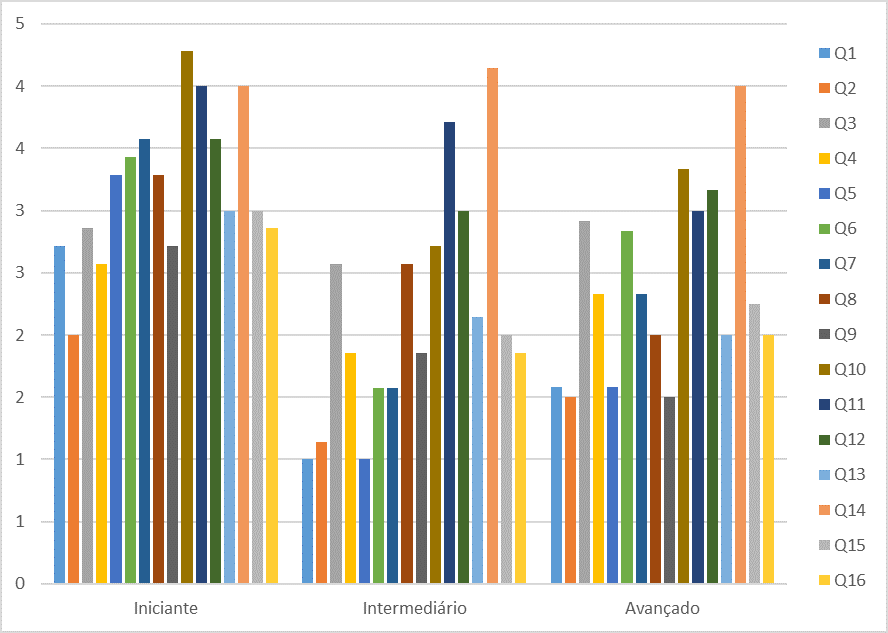
\includegraphics[width=0.9\textwidth]{./04-figuras/graph_scaleMean}
	\fonte{próprio autor}
	\label{fig:graph_scaleMean}
\end{figure}

Podemos notar a proximidade das respostas dos níveis intermediário e avançado, mas ainda assim as médias do nível avançado são ligeiramente maiores que as do nível intermediário. Essa diferença pode ser explicada pela experiência dos respondentes, muitas vezes conhecer as características da linguagem não significa tempo de experiência.

Os pesos de cada critério foi identificado a partir da média ponderada de cada questão, para evitar que o peso de cada resposta fosse completamente dependente das respostas dos respondentes identificados como iniciantes.

Pode-se verificar na \autoref{tab:tabelaPesos} os pesos calculados para cada um dos critérios de avaliação identificados.

\begin{table}[!htb]
	\centering
	\caption{Tabela com peso de cada critério avaliado.}
	\label{tab:tabelaPesos}
	\begin{tabular}{l|l}
		\textbf{Critério}                                                           & \textbf{Peso} \\ \hline
		Seletores raros: \{{[}\textasciicircum ={]}, {[}\$={]}, \char`~, +,\textgreater\} & 3             \\
		Agrupamentos                                                                & 2,8           \\
		Aninhamento                                                                 & 2,8           \\
		Propriedade simplificada                                                    & 3,2           \\
		Pseudo elementos                                                            & 2,8           \\
		Seletor com mais de 35 caracteres                                           & 3             \\
		At-rules                                                                    & 2,8           \\
		Media queries                                                               & 3,8           \\
		Prefixos: \{-webkit, -ms, etc.\}                                            & 4,2           \\
		Clausula :not                                                               & 3,8           \\
		Complexidade do seletor                                                     & 4,8           \\
		Seletor de localidade: \{nth-last-child, first-child, etc.\}                & 2,6          
	\end{tabular}
	\fonte{Próprio autor}
\end{table}

Esses foram os critérios de avaliação identificados para o cálculo da métrica. A partir desses pesos será feito a avaliação das folhas de estilo dos projetos open-source, para assim identificarmos uma escala para os valores encontrados para cada folha de estilo.